\textbf{内存特征}
\begin{description}
	\item[Location]CPU,内部,外部
	\item[Capacity]字大小,字数目
	\item[Unit of transfer]内部(一字),外部(多字) --- Addressable Unit: 内部(一字节),外部(簇)
	\item[Access method] 访存方式
		\begin{itemize}
			\item Sequential 串行访问 (tape)
			\item Direct 直接访问 (disk)
			\item Random 随机访问 (RAM,ROM)
			\item Associative 关联访问 (cache)
		\end{itemize}
	\item[Performance] 评价指标
		\begin{itemize}
			\item Access time
			\item Memory Cycle time
			\item Transfer Rate
		\end{itemize}
	\item[Physical type] 物理类型
		\begin{itemize}
			\item Semiconductor (RAM)
			\item Magnetic (disk \& tape)
			\item Optical (CD \& DVD)
			\item Others (Bubble Hologram)
		\end{itemize}
	\item[Organisation] Physical arrangement of bits into words(存储字)
\end{description}

\begin{table*}
	\begin{minipage}[b]{.5\linewidth}
	\centering
	\caption{RAM 区别}
	\begin{tabular}{|>{\bfseries}l|c|c|}
		\hline
		& \bfseries DRAM &\bfseries SRAM \\
		\hline
		字节存储方式 & 电容电荷 & 开关状态 \\
		电荷泄漏 & 有 & 无 \\
		刷新 & 需要 & 不需要 \\
		构造 & 简单 & 复杂 \\
		每位规模 & 更小 & 更大 \\
		价格 & 便宜 & 昂贵 \\
		刷新电路 & 需要 & 不需要 \\
		速度 & 更慢 & 更快 \\
		用途 & 主存储器 & 高速缓存 \\
		\hline
	\end{tabular}
	\end{minipage}
	\begin{minipage}[b]{.5\linewidth}
	\centering
	\caption{ROM 区别}
	\begin{tabular}{|>{\bfseries}p{10em}|p{8em}|}
		\hline
		掩膜型 ROM & 无法修改 \\
		\hline
		可编程只读存储器 PROM & 一旦写入,不可改变 \\
		\hline
		可擦除可编程只读存储器 EPROM & 可写,用紫外光擦除,重新写入 \\
		\hline
		点可擦除的可编程只读存储器 EEPROM & 通电擦除,重新写入 \\
		\hline
		闪存 Flash & 对芯片编程,通电擦除再写入 \\
		\hline
	\end{tabular}
	\end{minipage}
\end{table*}

\textbf{I/O数据传送方式}
\begin{description}
	\item[程序控制方式 Programmed I/O] CPU与外设之间的数据传送是在程序控制下完成的。用查询方式使 CPU 与外设交换数据时,CPU要不断读取状态位,检查输入设备是否已准备好数据。由于许多外设的速度很低,这种等待过程会占去CPU的绝大部分时间,而真正用于传输数据的时间却很少,使CPU的利用率变得很低。
	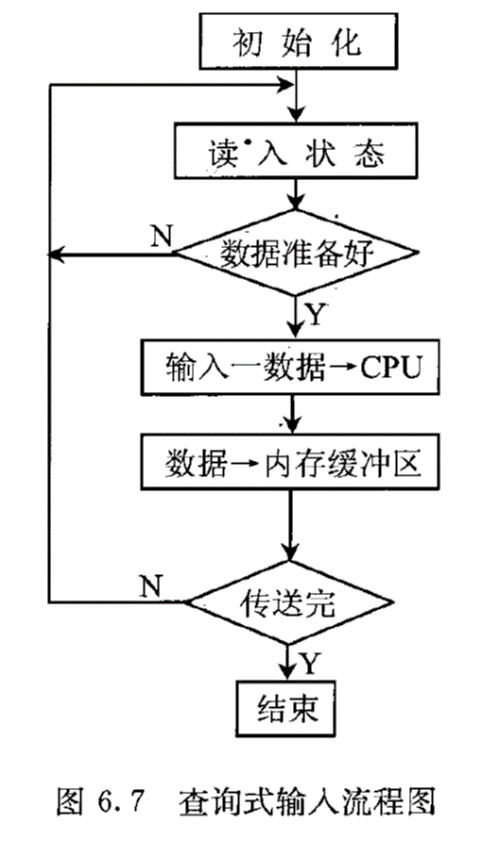
\includegraphics[width=0.75\columnwidth]{pinput.png}
	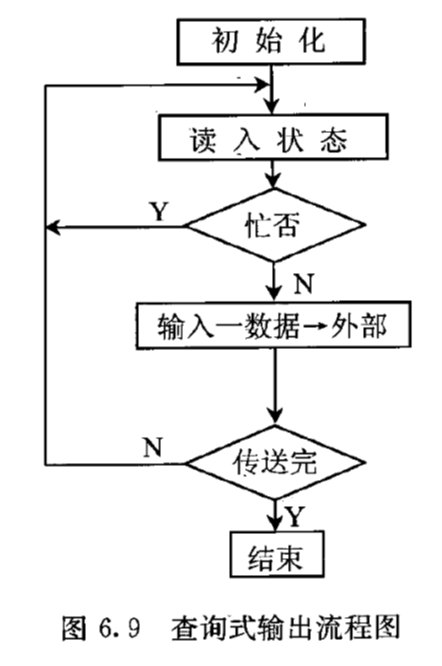
\includegraphics[width=0.75\columnwidth]{poutput.png}
	\item[中断方式 Interrupt driven I/O]采用中断方式后,CPU平时可以执行主程序,只有当输入设备将数据准备好了,或者输出端口的数据缓冲器已空时,才向CPU发中断请求。CPU响应中断后,暂停执行当前的程序,转去执行管理外设的中断服务程序(ISR)。在中断服务程序中,用于输入或输出指令在CPU和外设之间进行一次数据交换。等输入或输出操作完成之后,CPU又回去执行原来的程序。
	\begin{figure}[H]
	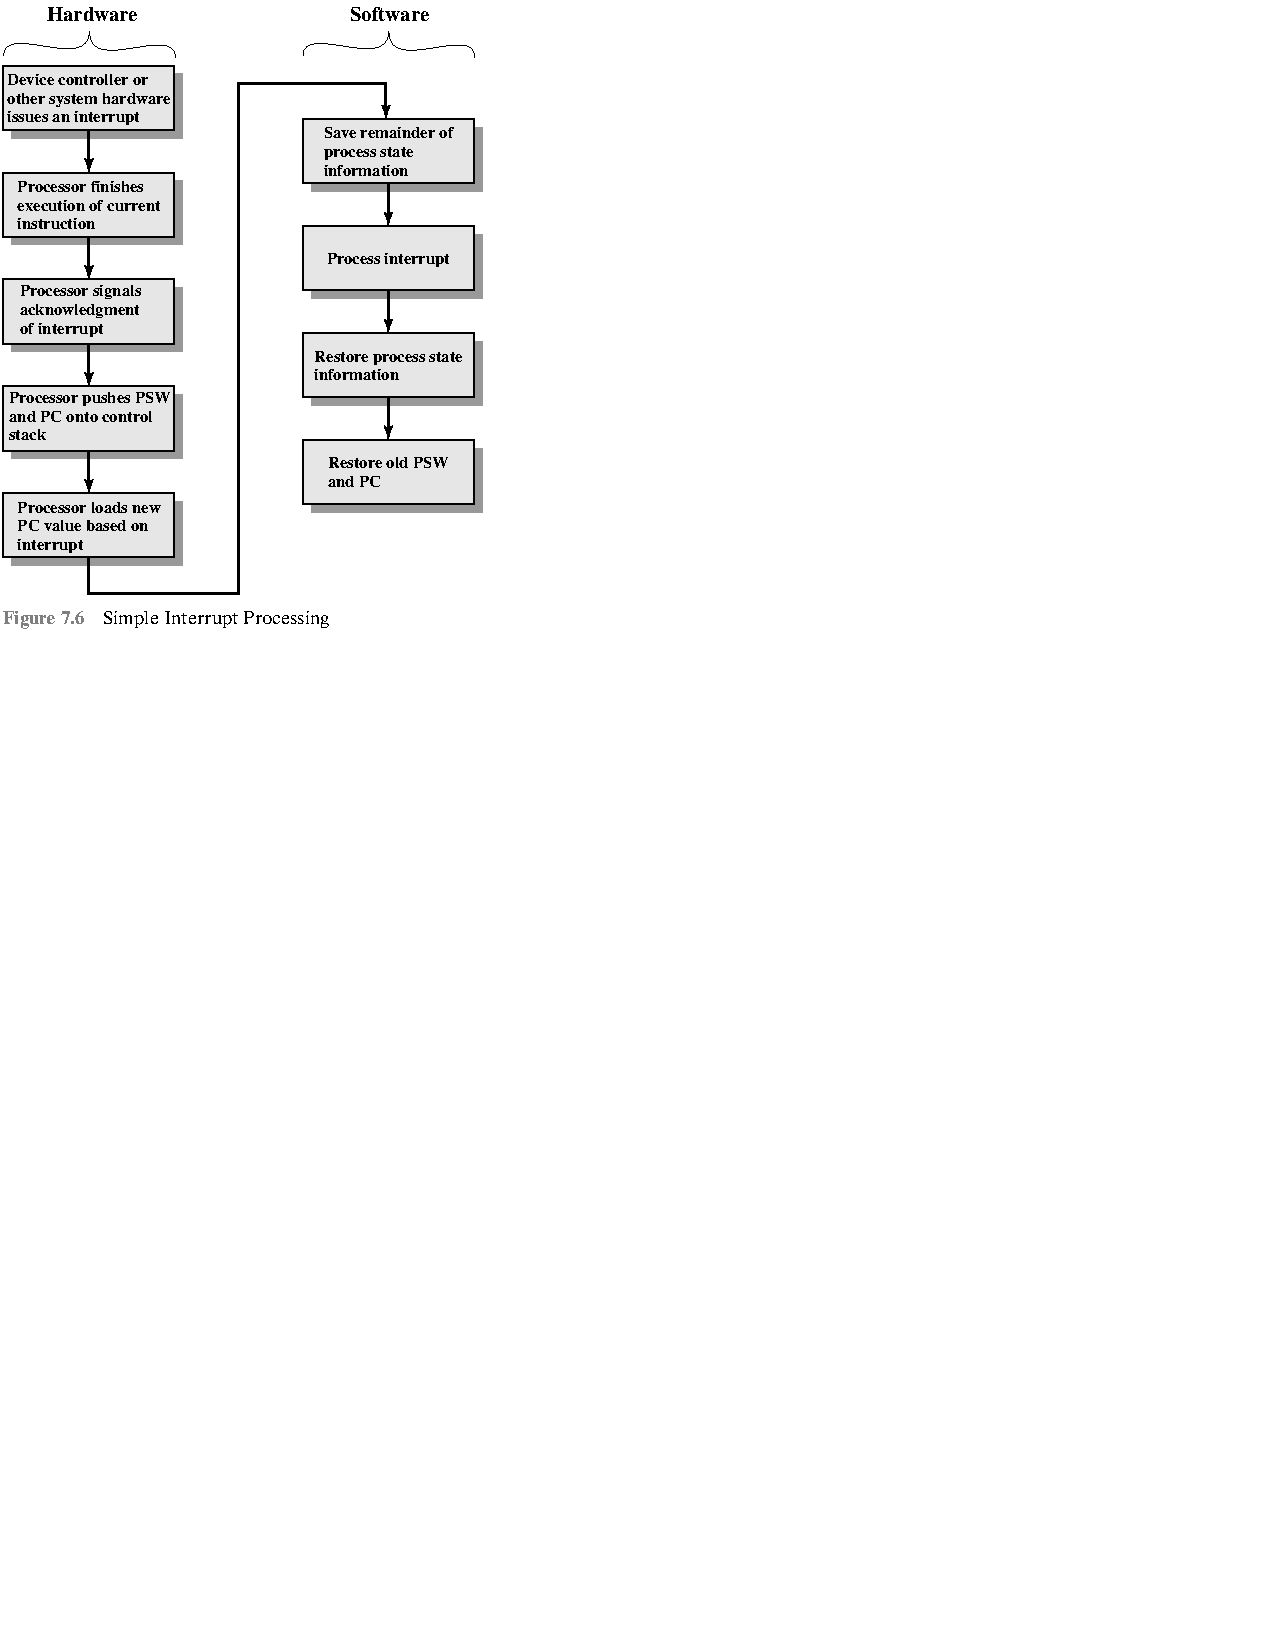
\includegraphics[width=\columnwidth]{interio.pdf}
	\end{figure}
	\item[直接存储器访问 DMA] DMA控制器临时接管总线,控制外设和存储器之间进行高速的数据传送,快速完成交换一批数据的任务,而不要CPU进行干预。这种控制器能给访问内存所需要的地址信息,并且能够自动修改地址指针,也能够设定和修改传送的字节数,还能够向存储器和外设发出相应的读写控制信号。在DMA传送结束后,它能够释放总线,把对总线的控制权又交还给CPU。
	\begin{figure}[H]
	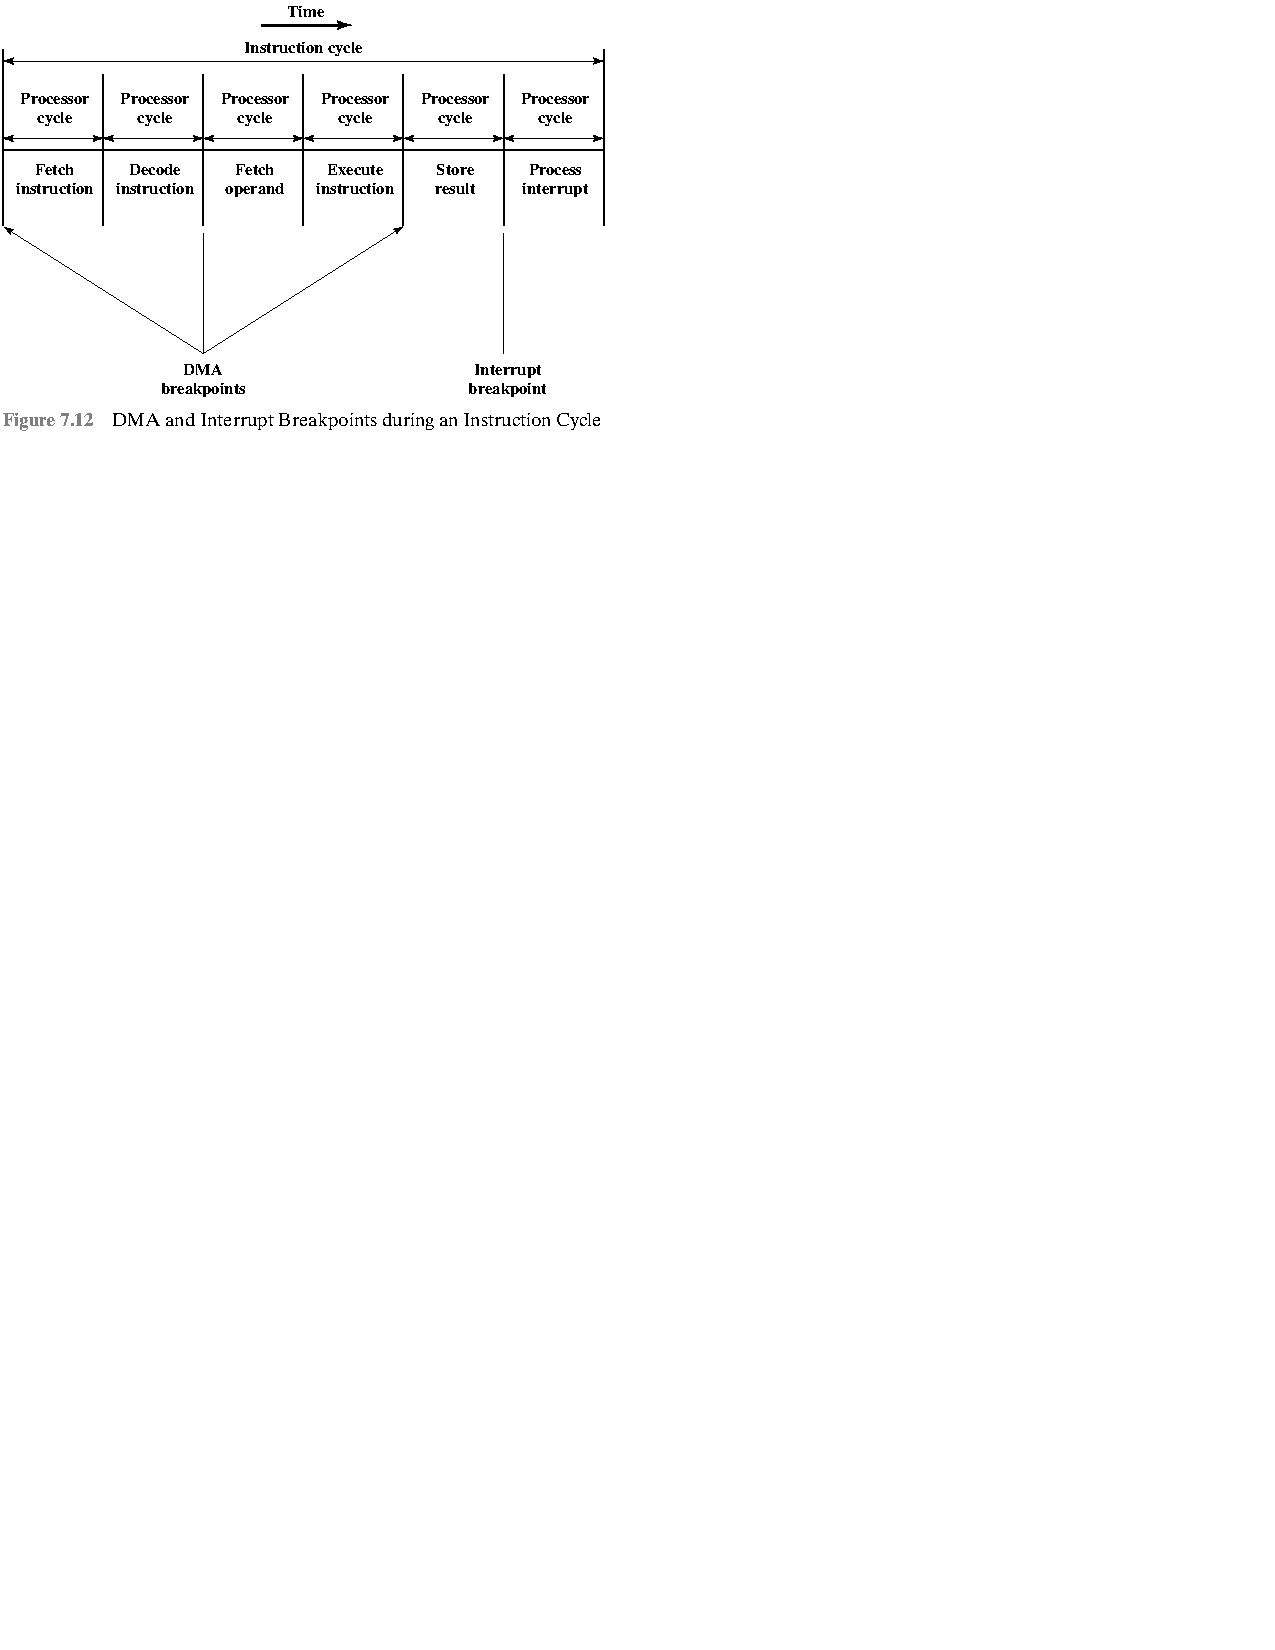
\includegraphics[width=\columnwidth]{DMA.pdf}
	\end{figure}
\end{description}

\begin{table*}
	\centering
	\caption{DMA 架构}
	\begin{tabular}{|>{\bfseries}l|c|c|}
		\hline
		& \bfseries 使用总线次数 &\bfseries CPU暂停次数 \\
		\hline
		Single Bus, Detached & 2 & 2 \\
		Single Bus,Intergrated & 1 & 1 \\
		Seperate I/O & 1 & 1 \\
		\hline
	\end{tabular}
\end{table*}
